\section{Generating a Mesh from an INP file}

Now that the system preferences have been adjusted to include AssyGen, Cubit, and CoreGen, you can generate a mesh by opening an INP file and though the \ui{Run MeshKit RGG dialog} accessed through the \ui{tools menu}.  Note the ``x" icon in the third column of the assemblies and core in the \ui{inputs panel}.  This designates that RGG believes that these components need to be meshed.

\begin{figure}[H]
	\begin{center}
		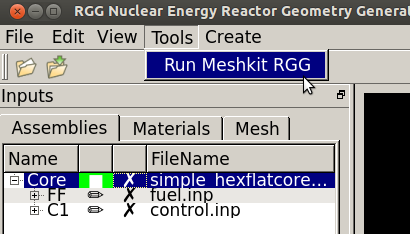
\includegraphics[width=0.5\linewidth]{Images/mesh-3.png}
		\caption{Opening the Run MeshKit RGG dialog.  The \ui{x icon}s denote that the FF and C1 assemblies need to be meshed.}
		\label{fig:Mesh3}
	\end{center}
\end{figure}

You will be prompted to save changes before proceeding if what is loaded into RGG differs from its file on disk.

The dialog should be populated with the assemblies that need to be re-meshed automatically.  In the example below, two assemblies need to be meshed, which also means that the core must be remeshed.  If ``Keep Going on Error" is checked, RGG will process every possible Assembly Files after an error occurs.  Any job that depends on the erred job will not be run.  If it is not checked, RGG will quite processing after the first error.  Checking ``Keep Going on Error" is advised if there are a large number of files to be processed.

\begin{figure}[H]
	\begin{center}
		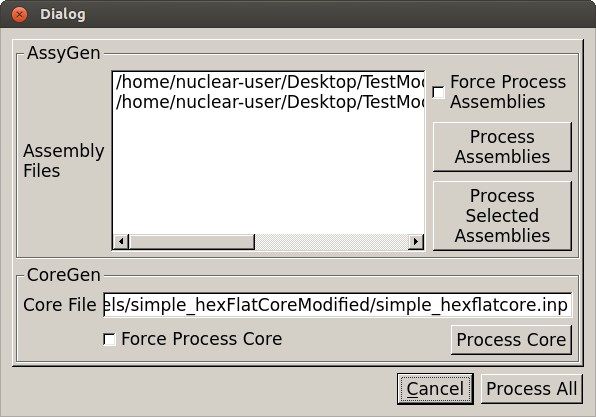
\includegraphics[width=0.5\linewidth]{Images/mesh-4.png}
		\caption{The Run MeshKit RGG dialog.}
		\label{fig:Mesh4}
	\end{center}
\end{figure}

One can force the generation of meshes regardless of their current state by using the \ui{force process assemblies checkbox} and the \ui{force process core checkbox} for an assembly or core, respectively.  To mesh both the core and assemblies, check both boxes and use the \ui{process all button}.  This is useful in cases where the exporting executables have changed.  A window that gives you the status of the processing should come up, similar to the shown in Figure \ref{fig:Mesh5}:

\begin{figure}[H]
	\begin{center}
		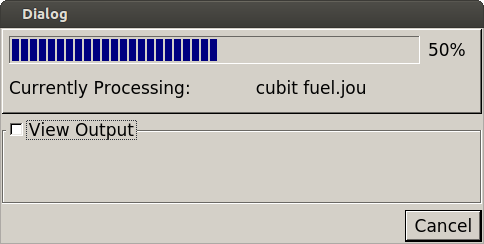
\includegraphics[width=0.5\linewidth]{Images/mesh-5.png}
		\caption{Running meshing.}
		\label{fig:Mesh5}
	\end{center}
\end{figure}

You can see the output of AssyGen, CoreGen, and Cubit by clicking on the \ui{view output checkbox}.  To cancel the current export, click the \ui{cancel button}.

To verify that the assemblies and core have been meshed, confirm that the \ui{x icon}s seen previously are now \ui{green square icon}s, as shown in Figure \ref{fig:Mesh6}.

\begin{figure}[H]
	\begin{center}
		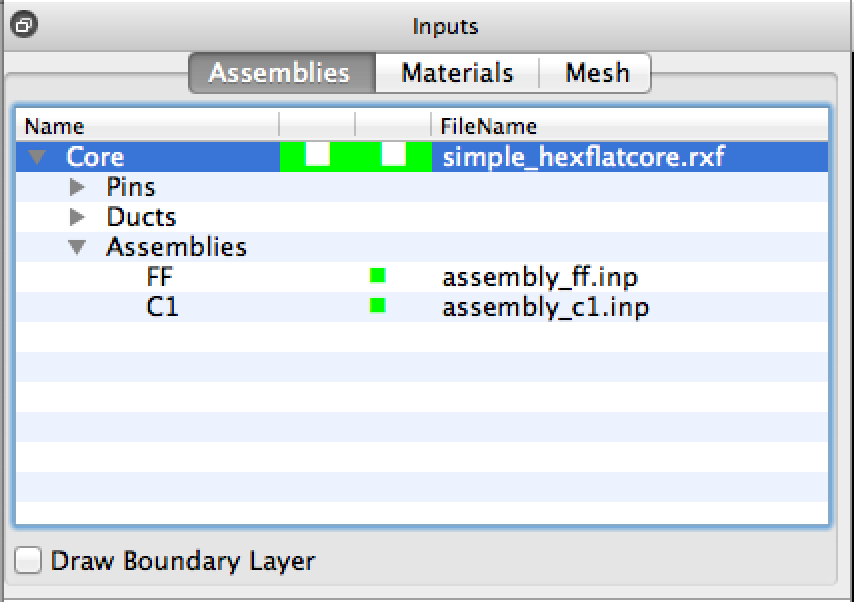
\includegraphics[width=0.5\linewidth]{Images/mesh-6.png}
		\caption{Verifying successful meshing.}
		\label{fig:Mesh6}
	\end{center}
\end{figure}

Note that the mesh needs to be loaded in after MeshKit creates it.  During this process, the tools menu is inaccessible.